\documentclass[border=10pt]{standalone}
\usepackage[svgnames]{xcolor}
\usepackage{amsmath}
\usepackage{pgfplots}
\pgfplotsset{compat=newest}
\usepackage[sfdefault]{FiraSans}
\usepackage{FiraMono}
\renewcommand*\familydefault{\sfdefault}
\begin{document}
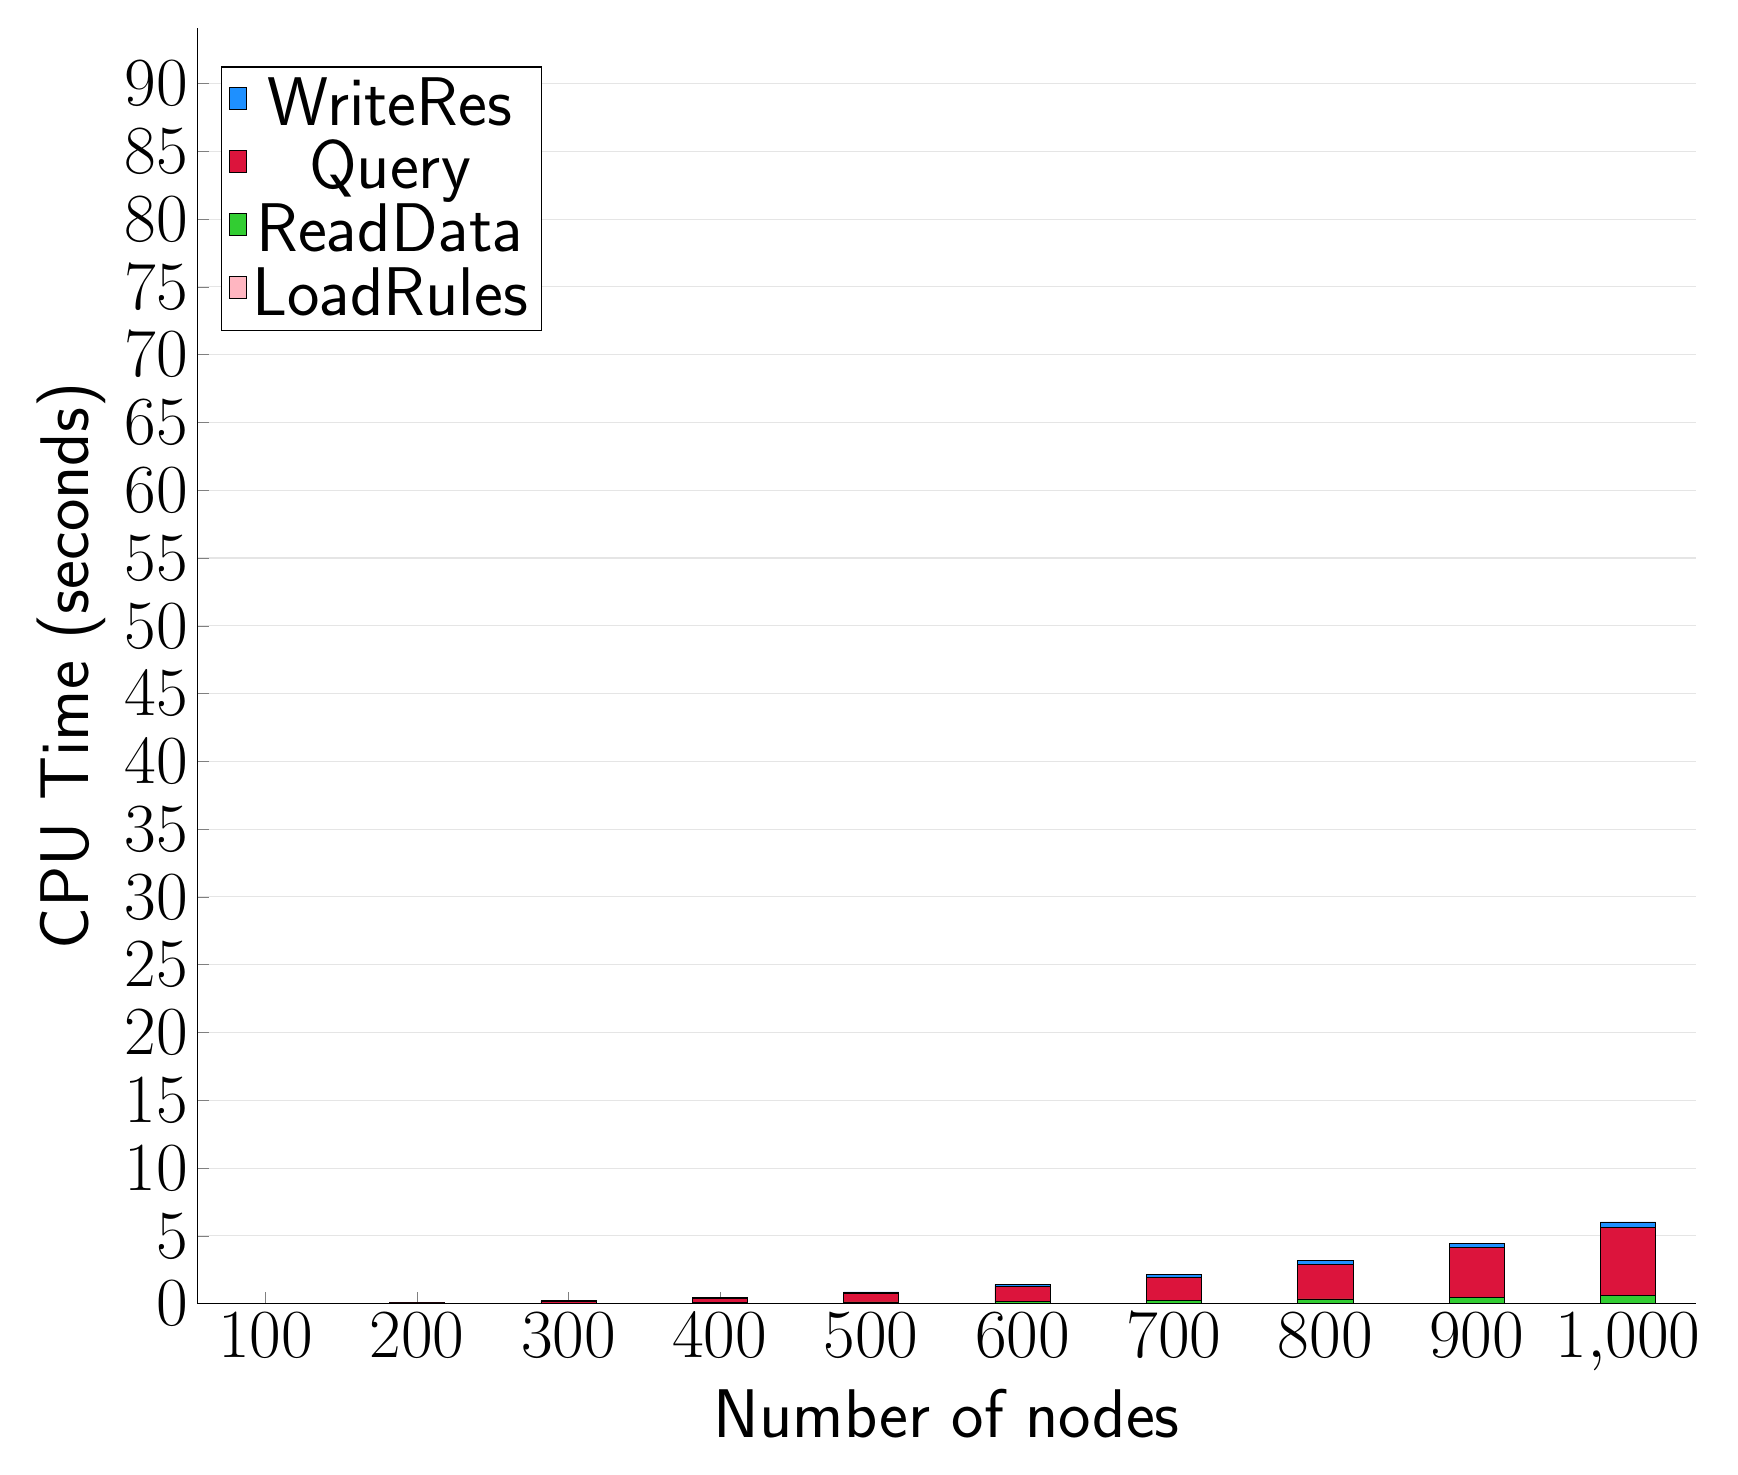
\begin{tikzpicture}
\begin{axis}[
   ybar stacked,
   width=1.7\textwidth,
   bar width=0.7cm,
   ymajorgrids, tick align=inside,
   major grid style={draw=gray!20},
   xtick=data,
   ymin=0, ymax=94.08204,
   axis x line*=bottom,
   axis y line*=left,
   enlarge x limits=0.05,
   legend style={
       at={(0.23, 0.97)},
       anchor=north east,
       legend columns=1,
       font=\Huge,
   },
   ylabel={CPU Time (seconds)},
   xlabel={Number of nodes},
   label style={font=\Huge},
   tick label style={font=\Huge},
]
\addlegendimage{fill=DodgerBlue, draw=black, line width=0.2pt}
\addlegendentry{WriteRes}
\addlegendimage{fill=Crimson, draw=black, line width=0.2pt}
\addlegendentry{Query}
\addlegendimage{fill=LimeGreen, draw=black, line width=0.2pt}
\addlegendentry{ReadData}
\addlegendimage{fill=LightPink, draw=black, line width=0.2pt}
\addlegendentry{LoadRules}
\addplot +[fill=LightPink, draw=black, line width=0.2pt] coordinates {
(100, 0.000547)
(200, 0.0005527999999999998)
(300, 0.0005453999999999996)
(400, 0.0005456000000000009)
(500, 0.0005463999999999998)
(600, 0.000547799999999999)
(700, 0.0005491999999999996)
(800, 0.0005476000000000002)
(900, 0.0005388000000000001)
(1000, 0.0005492000000000002)
};
\addplot +[fill=LimeGreen, draw=black, line width=0.2pt] coordinates {
(100, 0.0040349999999999995)
(200, 0.0169408)
(300, 0.039872399999999995)
(400, 0.0743898)
(500, 0.12167779999999999)
(600, 0.1819734)
(700, 0.2590598)
(800, 0.3531926)
(900, 0.4652198)
(1000, 0.6027292)
};
\addplot +[fill=Crimson, draw=black, line width=0.2pt] coordinates {
(100, 0.0053082)
(200, 0.0414406)
(300, 0.13832039999999998)
(400, 0.3222674)
(500, 0.6293390000000001)
(600, 1.0751302)
(700, 1.7041456)
(800, 2.5593396)
(900, 3.655734)
(1000, 5.021369)
};
\addplot +[fill=DodgerBlue, draw=black, line width=0.2pt] coordinates {
(100, 0.00412)
(200, 0.017191799999999997)
(300, 0.036710999999999994)
(400, 0.06583419999999998)
(500, 0.10668700000000002)
(600, 0.15758059999999996)
(700, 0.19956759999999996)
(800, 0.25718620000000014)
(900, 0.32747080000000006)
(1000, 0.4123279999999999)
};
\end{axis}
\end{tikzpicture}

\end{document}
